\documentclass[12pt,a4paper]{article}

% === Packages ===
\usepackage[T1]{fontenc}
\usepackage[utf8]{inputenc}
\usepackage[margin=2.5cm]{geometry}
\usepackage{hyperref}
\usepackage{amsmath}
\usepackage{amssymb}
\usepackage{graphicx}
\usepackage{booktabs}
\usepackage{listings}
\usepackage{xcolor}
\usepackage[ruled,vlined,linesnumbered]{algorithm2e}
\usepackage{float}
\usepackage{caption}
\usepackage{subcaption}
\usepackage{enumitem}
\usepackage{multirow}
\usepackage{array}
\usepackage{fancyhdr}
\usepackage{titlesec}

% === En-tete / Pied de page ===
\pagestyle{fancy}
\fancyhf{}
\fancyhead[L]{\small\textit{Moteur de Recherche S\'{e}mantique -- pgvector}}
\fancyhead[R]{\small\textit{ZIADI \& BOUKAKIOU}}
\fancyfoot[C]{\thepage}
\renewcommand{\headrulewidth}{0.4pt}

% === Configuration listings ===
\definecolor{codegreen}{rgb}{0,0.6,0}
\definecolor{codegray}{rgb}{0.5,0.5,0.5}
\definecolor{codepurple}{rgb}{0.58,0,0.82}
\definecolor{backcolour}{rgb}{0.96,0.96,0.96}
\definecolor{keyblue}{rgb}{0.13,0.29,0.53}

\lstdefinestyle{mystyle}{
    backgroundcolor=\color{backcolour},
    commentstyle=\color{codegreen}\itshape,
    keywordstyle=\color{keyblue}\bfseries,
    numberstyle=\tiny\color{codegray},
    stringstyle=\color{codepurple},
    basicstyle=\ttfamily\footnotesize,
    breaklines=true,
    numbers=left,
    numbersep=5pt,
    frame=single,
    tabsize=2,
    captionpos=b,
    aboveskip=10pt,
    belowskip=8pt,
}
\lstset{style=mystyle}

% === Hyperliens ===
\hypersetup{
    colorlinks=true,
    linkcolor=keyblue,
    citecolor=keyblue,
    urlcolor=codepurple,
}

% === Metadonnees ===
\title{
    \vspace{-1cm}
    \rule{\textwidth}{1.5pt}\\[0.4cm]
    \textbf{\LARGE Conception et Impl\'{e}mentation d'un\\Moteur de Recherche S\'{e}mantique}\\[0.3cm]
    \large Bas\'{e} sur PostgreSQL + pgvector\\[0.3cm]
    \rule{\textwidth}{1.5pt}\\[0.5cm]
    \normalsize Mini-projet -- Bases de Donn\'{e}es Avanc\'{e}es\\
    \'{E}cole nationale Sup\'{e}rieure d'Informatique (ESI) -- Alger\\
    2CS SIQ1 -- Ann\'{e}e universitaire 2025--2026
}
\author{
    Idriss Yacine ZIADI \and Rayan BOUKAKIOU
}
\date{Juin 2026}

\begin{document}

\maketitle
\thispagestyle{empty}

\begin{abstract}
\noindent
Ce rapport pr\'{e}sente la conception et l'impl\'{e}mentation d'un moteur de recherche s\'{e}mantique capable de retrouver des documents par leur \textit{sens} plut\^{o}t que par correspondance lexicale. Le syst\`{e}me repose sur l'extension \textbf{pgvector} de PostgreSQL~16 pour le stockage et l'indexation vectorielle, et sur le mod\`{e}le \textbf{all-MiniLM-L6-v2} (Sentence-Transformers) pour la g\'{e}n\'{e}ration d'embeddings \`{a} 384~dimensions. \'{E}valu\'{e} sur un corpus de 1\,964~articles de presse (AG~News), le moteur s\'{e}mantique atteint une Precision@5 de \textbf{0.81} contre 0.76 pour la m\'{e}thode TF-IDF de r\'{e}f\'{e}rence, avec un temps de r\'{e}ponse moyen de 19.8~ms. Une API REST (FastAPI) compl\`{e}te le dispositif.\\[0.2cm]
\textbf{Mots-cl\'{e}s :} recherche s\'{e}mantique, bases de donn\'{e}es vectorielles, pgvector, embeddings, Sentence-Transformers, HNSW, TF-IDF, PostgreSQL.
\end{abstract}

\newpage
\tableofcontents
\newpage

% ================================================================
% SECTION 1 : INTRODUCTION
% ================================================================
\section{Introduction}

\subsection{Contexte et motivation}

La recherche d'information constitue un d\'{e}fi fondamental de l'\`{e}re num\'{e}rique. Les syst\`{e}mes traditionnels de recherche par mots-cl\'{e}s, fond\'{e}s sur la correspondance lexicale exacte, pr\'{e}sentent des limitations majeures :
\begin{itemize}[noitemsep]
    \item \textbf{Sensibilit\'{e} aux synonymes} : les termes ``crise financi\`{e}re'' et ``effondrement \'{e}conomique'' d\'{e}signent le m\^{e}me ph\'{e}nom\`{e}ne mais ne partagent aucun mot ;
    \item \textbf{D\'{e}pendance \`{a} la formulation} : une l\'{e}g\`{e}re reformulation de la requ\^{e}te peut modifier radicalement les r\'{e}sultats ;
    \item \textbf{Incapacit\'{e} s\'{e}mantique} : la correspondance par termes ne capture pas le \textit{sens} sous-jacent d'un texte.
\end{itemize}

Face \`{a} ces limites, les approches de \textit{recherche s\'{e}mantique} transforment les textes en vecteurs num\'{e}riques (embeddings) dans un espace continu o\`{u} la proximit\'{e} g\'{e}om\'{e}trique refl\`{e}te la similarit\'{e} de sens.

\subsection{Probl\'{e}matique}

\textit{Comment concevoir et impl\'{e}menter un syst\`{e}me capable de retrouver des documents par leur sens plut\^{o}t que par la correspondance exacte de mots-cl\'{e}s, en s'appuyant sur des technologies open-source ?}

\subsection{Objectifs p\'{e}dagogiques}

Ce mini-projet vise \`{a} d\'{e}velopper les comp\'{e}tences suivantes :
\begin{enumerate}[noitemsep]
    \item Comprendre le fonctionnement des bases de donn\'{e}es vectorielles ;
    \item G\'{e}n\'{e}rer des repr\'{e}sentations vectorielles (embeddings) \`{a} partir de textes ;
    \item Concevoir une architecture compl\`{e}te de recherche s\'{e}mantique ;
    \item Impl\'{e}menter une recherche par similarit\'{e} (cosinus et L2) ;
    \item Comparer quantitativement recherche lexicale (TF-IDF) et recherche s\'{e}mantique ;
    \item R\'{e}diger un rapport technique structur\'{e}.
\end{enumerate}

\subsection{Technologies utilis\'{e}es}

Le syst\`{e}me repose exclusivement sur des technologies open-source :
\begin{itemize}[noitemsep]
    \item \textbf{PostgreSQL~16 + pgvector~0.7} \cite{pgvector2023} pour le stockage et l'indexation vectorielle ;
    \item \textbf{Sentence-Transformers} \cite{reimers2019sentence} (mod\`{e}le \texttt{all-MiniLM-L6-v2}) pour la g\'{e}n\'{e}ration d'embeddings ;
    \item \textbf{scikit-learn~1.4} pour l'impl\'{e}mentation TF-IDF de r\'{e}f\'{e}rence ;
    \item \textbf{FastAPI~0.111} pour l'exposition via API REST ;
    \item \textbf{Docker Compose} pour l'orchestration de l'infrastructure.
\end{itemize}

\subsection{Plan du rapport}

La section~\ref{sec:etat} pr\'{e}sente l'\'{e}tat de l'art. La section~\ref{sec:methodo} d\'{e}crit la m\'{e}thodologie et l'architecture. La section~\ref{sec:impl} d\'{e}taille l'impl\'{e}mentation. La section~\ref{sec:resultats} analyse les r\'{e}sultats exp\'{e}rimentaux. La section~\ref{sec:discussion} propose une discussion critique. Enfin, la section~\ref{sec:conclusion} conclut ce travail.

% ================================================================
% SECTION 2 : ETAT DE L'ART
% ================================================================
\section{\'{E}tat de l'art}
\label{sec:etat}

\subsection{De la recherche lexicale \`{a} la recherche s\'{e}mantique}

La recherche d'information a \'{e}volu\'{e} en trois grandes phases. La premi\`{e}re, la \textbf{recherche bool\'{e}enne}, repose sur des op\'{e}rateurs logiques (AND, OR, NOT) appliqu\'{e}s \`{a} des index invers\'{e}s. La deuxi\`{e}me, le \textbf{mod\`{e}le vectoriel TF-IDF} \cite{robertson2009bm25}, pond\`{e}re les termes par leur fr\'{e}quence et leur raret\'{e} dans le corpus. La troisi\`{e}me, la \textbf{recherche s\'{e}mantique}, projette les textes dans un espace vectoriel dense o\`{u} la proximit\'{e} g\'{e}om\'{e}trique encode la similarit\'{e} de sens.

\subsection{Bases de donn\'{e}es vectorielles}

Une base de donn\'{e}es vectorielle est un syst\`{e}me optimis\'{e} pour stocker et interroger des vecteurs dans un espace \`{a} haute dimension. Contrairement aux bases relationnelles qui op\`{e}rent sur des donn\'{e}es structur\'{e}es via SQL, les bases vectorielles permettent la recherche par \textit{proximit\'{e}} selon une m\'{e}trique de distance.

Le tableau~\ref{tab:vectordb} compare les principales solutions disponibles en 2024.

\begin{table}[H]
\centering
\caption{Comparaison des principales bases de donn\'{e}es vectorielles}
\label{tab:vectordb}
\begin{tabular}{@{}lccccc@{}}
\toprule
\textbf{Crit\`{e}re} & \textbf{pgvector} & \textbf{FAISS} & \textbf{Pinecone} & \textbf{ChromaDB} & \textbf{Milvus} \\
\midrule
Open-source        & Oui       & Oui    & Non       & Oui       & Oui \\
Int\'{e}gration SQL   & \textbf{Oui} & Non & Non    & Non       & Non \\
Index HNSW         & Oui       & Oui    & Oui       & Oui       & Oui \\
Index IVFFlat      & Oui       & Oui    & Non       & Non       & Oui \\
Scalabilit\'{e}       & \~{}10M   & \~{}1B & \~{}1B   & \~{}10M   & \~{}1B \\
Requ\^{e}tes hybrides & \textbf{Oui} & Non & Partiel & Non    & Oui \\
Licence            & PostgreSQL & MIT   & Propri\'{e}t. & Apache  & Apache \\
\bottomrule
\end{tabular}
\end{table}

\textbf{Justification du choix de pgvector.} pgvector s'int\`{e}gre nativement dans PostgreSQL, permettant de combiner recherche vectorielle et requ\^{e}tes SQL classiques dans une m\^{e}me transaction. Cette capacit\'{e} de \textit{requ\^{e}te hybride} (filtrage m\'{e}tadonn\'{e}es + recherche vectorielle) est un avantage d\'{e}terminant pour les cas d'usage r\'{e}els. De plus, PostgreSQL b\'{e}n\'{e}ficie d'un \'{e}cosyst\`{e}me mature (sauvegardes, r\'{e}plication, monitoring) qui facilite la mise en production.

\subsection{Repr\'{e}sentations vectorielles (Embeddings)}

Les repr\'{e}sentations vectorielles transforment du texte en vecteurs num\'{e}riques dans un espace continu. On distingue deux g\'{e}n\'{e}rations :

\textbf{Embeddings statiques.} Word2Vec (Mikolov et al., 2013) et GloVe (Pennington et al., 2014) produisent un vecteur \textit{unique} par mot, ind\'{e}pendant du contexte. Le mot ``banque'' aura le m\^{e}me vecteur qu'il d\'{e}signe un \'{e}tablissement financier ou le bord d'une rivi\`{e}re. Pour repr\'{e}senter une phrase, on recourt typiquement \`{a} la moyenne des vecteurs de mots, ce qui perd l'information d'ordre et de syntaxe.

\textbf{Embeddings contextuels.} BERT (Devlin et al., 2019) et ses d\'{e}riv\'{e}s produisent des repr\'{e}sentations contextuelles au niveau du \textit{token}. Sentence-Transformers \cite{reimers2019sentence} adapte cette architecture pour produire des embeddings au niveau de la \textit{phrase enti\`{e}re} via un r\'{e}seau siamois. Le mod\`{e}le \texttt{all-MiniLM-L6-v2} utilis\'{e} dans ce projet offre les caract\'{e}ristiques suivantes :

\begin{table}[H]
\centering
\caption{Caract\'{e}ristiques du mod\`{e}le all-MiniLM-L6-v2}
\label{tab:model}
\begin{tabular}{@{}ll@{}}
\toprule
\textbf{Propri\'{e}t\'{e}} & \textbf{Valeur} \\
\midrule
Dimension de sortie     & 384 \\
Nombre de param\`{e}tres  & 22.7~millions \\
Longueur max. d'entr\'{e}e & 256 tokens \\
Taille du mod\`{e}le       & 80~MB \\
Vitesse (CPU)            & \~{}2\,800 phrases/s \\
Score STS Benchmark      & 0.8282 (Pearson) \\
\bottomrule
\end{tabular}
\end{table}

\subsection{M\'{e}triques de similarit\'{e}}

La \textbf{similarit\'{e} cosinus} mesure l'angle entre deux vecteurs, ind\'{e}pendamment de leur norme :
\begin{equation}
\text{sim}_{\cos}(\vec{u}, \vec{v}) = \frac{\vec{u} \cdot \vec{v}}{||\vec{u}|| \cdot ||\vec{v}||} = \frac{\sum_{i=1}^{n} u_i v_i}{\sqrt{\sum_{i=1}^{n} u_i^2} \cdot \sqrt{\sum_{i=1}^{n} v_i^2}}
\label{eq:cosine}
\end{equation}

La \textbf{distance euclidienne} (L2) mesure la distance g\'{e}om\'{e}trique directe :
\begin{equation}
d_{L2}(\vec{u}, \vec{v}) = \sqrt{\sum_{i=1}^{n}(u_i - v_i)^2}
\label{eq:l2}
\end{equation}

Pour des vecteurs \textit{normalis\'{e}s} ($||\vec{u}|| = ||\vec{v}|| = 1$), on a la relation $d_{L2}^2 = 2(1 - \text{sim}_{\cos})$, ce qui rend les deux m\'{e}triques \'{e}quivalentes en termes de classement. C'est pourquoi notre pipeline utilise \texttt{normalize\_embeddings=True}.

\subsection{Indexation vectorielle : HNSW vs IVFFlat}

La recherche exacte par force brute (scan s\'{e}quentiel) a une complexit\'{e} $O(n \cdot d)$. Pour des collections de grande taille, des \textit{index approximatifs} (ANN -- Approximate Nearest Neighbors) sont indispensables.

\textbf{HNSW} (Hierarchical Navigable Small World) \cite{malkov2020hnsw} construit un graphe multi-couches o\`{u} chaque couche est un sous-graphe navigable de la pr\'{e}c\'{e}dente. La recherche s'effectue en $O(\log n)$ en descendant depuis la couche la plus clairsem\'{e}e. Les param\`{e}tres cl\'{e}s sont :
\begin{itemize}[noitemsep]
    \item $m$ : nombre de connexions bidirectionnelles par n\oe ud. Une valeur \'{e}lev\'{e}e am\'{e}liore le recall mais augmente la m\'{e}moire ;
    \item $ef\_construction$ : taille de la liste de candidats lors de la construction. Contr\^{o}le le compromis temps de construction / qualit\'{e}.
\end{itemize}

\textbf{IVFFlat} (Inverted File with Flat quantization) partitionne l'espace en cellules de Vorono\"{\i} via k-means. Lors d'une requ\^{e}te, seules les $n_{probes}$ cellules les plus proches sont explor\'{e}es. La complexit\'{e} est $O(\sqrt{n})$.

\begin{table}[H]
\centering
\caption{Comparaison d\'{e}taill\'{e}e HNSW vs IVFFlat dans pgvector}
\label{tab:index}
\begin{tabular}{@{}lcc@{}}
\toprule
\textbf{Crit\`{e}re} & \textbf{HNSW} & \textbf{IVFFlat} \\
\midrule
Complexit\'{e} recherche  & $O(\log n)$     & $O(\sqrt{n})$ \\
Recall@10 typique       & $\geq 99\%$     & $\sim 95\%$ \\
M\'{e}moire par vecteur     & $\sim 1.5\times$ & $1\times$ (base) \\
Temps de construction    & \'{E}lev\'{e}         & Mod\'{e}r\'{e} \\
Mise \`{a} jour incr\'{e}mentale & Oui           & Non (reconstruction) \\
Param\`{e}tres critiques    & $m$, $ef\_construction$ & $lists$, $probes$ \\
Cas d'usage recommand\'{e} & $< 5$M vecteurs & $> 5$M vecteurs \\
Op\'{e}rateur pgvector     & \texttt{vector\_cosine\_ops} & \texttt{vector\_cosine\_ops} \\
\bottomrule
\end{tabular}
\end{table}

Pour notre corpus de 1\,964~documents, HNSW avec $m=16$ et $ef\_construction=64$ est le choix optimal : recall quasi-parfait, construction rapide (\`{a} cette \'{e}chelle), et support des mises \`{a} jour incr\'{e}mentales.

\subsection{TF-IDF et BM25 : m\'{e}thodes de r\'{e}f\'{e}rence}

Le mod\`{e}le TF-IDF \cite{robertson2009bm25} assigne \`{a} chaque terme $t$ dans un document $d$ un poids :
\begin{equation}
\text{tf-idf}(t, d) = \text{tf}(t, d) \times \log \frac{|D|}{\text{df}(t) + 1}
\label{eq:tfidf}
\end{equation}

o\`{u} $\text{tf}(t,d)$ est la fr\'{e}quence du terme, $|D|$ le nombre total de documents, et $\text{df}(t)$ le nombre de documents contenant $t$. Le document est ainsi repr\'{e}sent\'{e} par un vecteur \textit{creux} (sparse) de grande dimension ($|V|$ = taille du vocabulaire).

BM25 (Best Matching 25) raffine TF-IDF en introduisant une saturation de la fr\'{e}quence et une normalisation par la longueur du document. Ces m\'{e}thodes restent des approches purement \textit{lexicales} : elles ne capturent pas la synonymie ni la paraphrase.

% ================================================================
% SECTION 3 : METHODOLOGIE
% ================================================================
\section{M\'{e}thodologie}
\label{sec:methodo}

\subsection{Architecture g\'{e}n\'{e}rale du syst\`{e}me}

L'architecture suit un pattern pipeline en cinq phases, de l'acquisition des donn\'{e}es brutes \`{a} la restitution des r\'{e}sultats (figure~\ref{fig:archi}).

\begin{figure}[H]
\centering
\fbox{\parbox{0.92\textwidth}{\small
\begin{verbatim}
  +------------------+      +-------------------+      +---------------------+
  |   AG News        |----->|   Preprocessing   |----->|  Sentence-Transformers
  |   (2000 docs)    |      |   - clean URLs    |      |  all-MiniLM-L6-v2   |
  |   Hugging Face   |      |   - normalize     |      |  384D, normalized   |
  +------------------+      |   - truncate 512  |      +----------+----------+
                             +-------------------+                 |
                                                          embeddings (2000x384)
                                                                   |
  +------------------+      +-------------------+      +-----------v----------+
  |   Top-K Results  |<-----|   Search Engine   |<-----|  PostgreSQL 16       |
  |   + similarity   |      |   - cosine / L2   |      |  + pgvector          |
  |   scores         |      |   - TF-IDF comp.  |      |  + HNSW index        |
  +------------------+      +-------------------+      |  (1964 docs stored)  |
          |                         ^                   +----------------------+
          v                         |
  +------------------+      +-------------------+
  |   FastAPI REST   |      |   Evaluation      |
  |   /search/*      |      |   P@k, temps,     |
  |   /health        |      |   figures         |
  +------------------+      +-------------------+
\end{verbatim}
}}
\caption{Architecture g\'{e}n\'{e}rale du syst\`{e}me de recherche s\'{e}mantique}
\label{fig:archi}
\end{figure}

\subsection{Choix du dataset}

Le dataset \textbf{AG News} est un corpus de 120\,000~articles de presse annot\'{e}s en 4~cat\'{e}gories. Nous utilisons les 2\,000~premiers articles du split d'entra\^{\i}nement, t\'{e}l\'{e}charg\'{e}s via la biblioth\`{e}que \texttt{datasets} de Hugging Face.

\begin{table}[H]
\centering
\caption{Statistiques du dataset apr\`{e}s pr\'{e}traitement}
\label{tab:dataset}
\begin{tabular}{@{}lr@{}}
\toprule
\textbf{Statistique} & \textbf{Valeur mesur\'{e}e} \\
\midrule
Documents t\'{e}l\'{e}charg\'{e}s   & 2\,000 \\
Documents uniques en base & 1\,964 (36 doublons filtr\'{e}s) \\
Cat\'{e}gorie World          & 477 (23.9\%) \\
Cat\'{e}gorie Sci/Tech        & 777 (38.9\%) \\
Cat\'{e}gorie Sports          & 338 (16.9\%) \\
Cat\'{e}gorie Business        & 408 (20.4\%) \\
Longueur moyenne            & 39.6 mots / 317 caract\`{e}res \\
Longueur m\'{e}diane           & 39 mots \\
Longueur maximale           & 134 mots \\
\bottomrule
\end{tabular}
\end{table}

Ce dataset est adapt\'{e} pour trois raisons : (1)~les cat\'{e}gories th\'{e}matiques sont distinctes, ce qui permet une \'{e}valuation quantitative via Precision@k ; (2)~les textes sont courts, correspondant au cas d'usage typique ; (3)~le d\'{e}s\'{e}quilibre mod\'{e}r\'{e} des classes (Sci/Tech 38.9\% vs Sports 16.9\%) permet de tester la robustesse des m\'{e}thodes.

\subsection{Pipeline de traitement}

\begin{table}[H]
\centering
\caption{D\'{e}tail du pipeline d'ex\'{e}cution (mesures r\'{e}elles sur CPU Intel)}
\label{tab:pipeline}
\begin{tabular}{@{}clrl@{}}
\toprule
\textbf{\#} & \textbf{\'{E}tape} & \textbf{Dur\'{e}e} & \textbf{D\'{e}tail} \\
\midrule
1 & T\'{e}l\'{e}chargement AG News   & 20.3s & via \texttt{datasets} (Hugging Face) \\
2 & Pr\'{e}traitement             & 0.1s  & Nettoyage, filtrage, troncature \\
3 & G\'{e}n\'{e}ration embeddings   & $\sim$120s & 2\,000 textes, batch=32, CPU \\
4 & Cr\'{e}ation sch\'{e}ma SQL      & 0.04s & 3 tables + contraintes \\
5 & Insertion documents         & 2.5s  & \texttt{execute\_values}, batch=100 \\
6 & Cr\'{e}ation index HNSW       & 0.6s  & $m=16$, $ef\_construction=64$ \\
7 & V\'{e}rification               & 0.01s & Comptage + inspection index \\
\midrule
  & \textbf{Total pipeline}     & \textbf{$\sim$144s} & \\
\bottomrule
\end{tabular}
\end{table}

\subsection{Protocole d'\'{e}valuation}

L'\'{e}valuation repose sur 20~requ\^{e}tes de test couvrant uniform\'{e}ment les 4~cat\'{e}gories (5~par cat\'{e}gorie). Pour chaque requ\^{e}te, la cat\'{e}gorie attendue est connue. La m\'{e}trique principale est la \textbf{Precision@k} :
\begin{equation}
P@k = \frac{|\{d \in \text{top-}k : \text{cat}(d) = \text{cat}_{\text{attendue}}\}|}{k}
\label{eq:patk}
\end{equation}

La Precision@k moyenne est calcul\'{e}e sur les 20~requ\^{e}tes pour $k \in \{1, 3, 5\}$, pour chacune des deux m\'{e}thodes (s\'{e}mantique et TF-IDF).

% ================================================================
% SECTION 4 : IMPLEMENTATION
% ================================================================
\section{Impl\'{e}mentation}
\label{sec:impl}

\subsection{Structure du projet}

Le code source est organis\'{e} en modules Python avec s\'{e}paration claire des responsabilit\'{e}s :

\begin{table}[H]
\centering
\caption{Modules du projet et leurs responsabilit\'{e}s}
\label{tab:modules}
\begin{tabular}{@{}llr@{}}
\toprule
\textbf{Module} & \textbf{Responsabilit\'{e}} & \textbf{Lignes} \\
\midrule
\texttt{config.py}          & Configuration centralis\'{e}e (.env)        & 20 \\
\texttt{data\_loader.py}    & T\'{e}l\'{e}chargement AG News              & 75 \\
\texttt{preprocessing.py}   & Nettoyage texte (URLs, emails, troncature) & 95 \\
\texttt{embeddings.py}      & G\'{e}n\'{e}ration embeddings (Sentence-Transformers) & 130 \\
\texttt{database.py}        & Connexion PostgreSQL, CRUD, pgvector       & 120 \\
\texttt{search.py}          & Recherche s\'{e}mantique + TF-IDF           & 150 \\
\texttt{evaluation.py}      & Benchmark P@k + g\'{e}n\'{e}ration figures  & 200 \\
\texttt{api.py}             & API REST FastAPI (5 endpoints)             & 120 \\
\texttt{schemas.py}         & Mod\`{e}les Pydantic                       & 35 \\
\midrule
\textbf{Total}              &                                            & \textbf{$\sim$945} \\
\bottomrule
\end{tabular}
\end{table}

\subsection{Sch\'{e}ma de la base de donn\'{e}es}

Le sch\'{e}ma comporte trois tables. La table principale \texttt{documents} est d\'{e}finie comme suit :

\begin{lstlisting}[language=SQL, caption={DDL de la table documents (extrait de \texttt{sql/01\_schema.sql})}]
CREATE EXTENSION IF NOT EXISTS vector;

CREATE TABLE IF NOT EXISTS documents (
    id SERIAL PRIMARY KEY,
    title TEXT NOT NULL,
    content TEXT NOT NULL,
    category VARCHAR(100),
    source VARCHAR(200) DEFAULT 'ag_news',
    char_count INTEGER,
    word_count INTEGER,
    embedding vector(384),  -- all-MiniLM-L6-v2
    created_at TIMESTAMP DEFAULT NOW(),
    CONSTRAINT uq_documents_title_source UNIQUE (title, source)
);
\end{lstlisting}

Le type \texttt{vector(384)} stocke un vecteur dense de 384~flottants. Les op\'{e}rateurs de distance sont :
\begin{itemize}[noitemsep]
    \item \texttt{<=>} : distance cosinus ($1 - \text{sim}_{\cos}$). Utilis\'{e} avec \texttt{vector\_cosine\_ops} ;
    \item \texttt{<->} : distance euclidienne (L2). Utilis\'{e} avec \texttt{vector\_l2\_ops}.
\end{itemize}

La contrainte \texttt{UNIQUE(title, source)} associ\'{e}e \`{a} \texttt{ON CONFLICT DO NOTHING} garantit l'\textit{idempotence} du pipeline : ex\'{e}cuter l'ingestion plusieurs fois ne cr\'{e}e pas de doublons.

La table \texttt{search\_logs} enregistre chaque requ\^{e}te avec son temps d'ex\'{e}cution, permettant un monitoring en production. La table \texttt{evaluation\_results} stocke les r\'{e}sultats des benchmarks.

\subsection{Indexation HNSW}

L'index HNSW acc\'{e}l\`{e}re la recherche de voisins proches :

\begin{lstlisting}[language=SQL, caption={Cr\'{e}ation de l'index HNSW (extrait de \texttt{sql/02\_indexes.sql})}]
CREATE INDEX IF NOT EXISTS idx_documents_embedding_hnsw
ON documents USING hnsw (embedding vector_cosine_ops)
WITH (m = 16, ef_construction = 64);
\end{lstlisting}

\subsection{Moteur de recherche s\'{e}mantique}

L'algorithme~\ref{alg:search} d\'{e}crit le processus de recherche s\'{e}mantique.

\begin{algorithm}[H]
\SetAlgoLined
\KwIn{Requ\^{e}te textuelle $q$, nombre de r\'{e}sultats $k$, m\'{e}trique $m$}
\KwOut{Liste de $k$ documents tri\'{e}s par similarit\'{e} d\'{e}croissante}
\BlankLine
$\vec{q} \leftarrow \text{SentenceTransformer.encode}(q, \text{normalize}=\text{True})$\;
\eIf{$m = \text{``cosine''}$}{
    $\text{op} \leftarrow \text{``<=>''}$ \tcp*{distance cosinus}
}{
    $\text{op} \leftarrow \text{``<->''}$ \tcp*{distance L2}
}
$R \leftarrow \text{SQL}(\text{SELECT id, title, content, category, } 1 - (\text{embedding} \; \text{op} \; \vec{q}) \; \text{FROM documents ORDER BY embedding} \; \text{op} \; \vec{q} \; \text{LIMIT} \; k)$\;
$\text{INSERT INTO search\_logs}(q, \vec{q}, k, m, \text{elapsed})$\;
\Return{$R$}
\caption{Recherche s\'{e}mantique via pgvector}
\label{alg:search}
\end{algorithm}

La requ\^{e}te SQL centrale est :

\begin{lstlisting}[language=SQL, caption={Requ\^{e}te de recherche s\'{e}mantique}]
SELECT id, title, content, category,
       1 - (embedding <=> %s::vector) AS similarity_score
FROM documents
ORDER BY embedding <=> %s::vector
LIMIT %s;
\end{lstlisting}

Le vecteur requ\^{e}te est pass\'{e} en param\`{e}tre \texttt{\%s} (et non par interpolation de cha\^{\i}ne) pour pr\'{e}venir les injections SQL.

\subsection{Comparaison avec TF-IDF}

L'impl\'{e}mentation TF-IDF utilise \texttt{TfidfVectorizer} de scikit-learn :
\begin{itemize}[noitemsep]
    \item \texttt{max\_features=50\,000} : limitation du vocabulaire pour \'{e}viter l'explosion dimensionnelle ;
    \item \texttt{ngram\_range=(1, 2)} : prise en compte des unigrammes et bigrammes ;
    \item Similarit\'{e} cosinus entre le vecteur requ\^{e}te et la matrice TF-IDF des documents.
\end{itemize}

La diff\'{e}rence fondamentale : TF-IDF repose sur la \textit{fr\'{e}quence des termes} (vecteurs creux, $\sim$50\,000 dimensions), tandis que les embeddings capturent le \textit{sens latent} (vecteurs denses, 384 dimensions).

\subsection{API REST (bonus)}

Une API FastAPI expose le moteur en tant que micro-service :

\begin{table}[H]
\centering
\caption{Endpoints de l'API REST}
\label{tab:api}
\begin{tabular}{@{}llp{6cm}@{}}
\toprule
\textbf{M\'{e}thode} & \textbf{Endpoint} & \textbf{Description} \\
\midrule
GET  & \texttt{/health}           & \'{E}tat de sant\'{e} (DB, nombre de docs, mod\`{e}le) \\
POST & \texttt{/search/semantic}  & Recherche s\'{e}mantique (cosinus ou L2) \\
POST & \texttt{/search/lexical}   & Recherche TF-IDF \\
POST & \texttt{/search/compare}   & Comparaison c\^{o}te-\`{a}-c\^{o}te + overlap \\
GET  & \texttt{/stats}            & Statistiques (temps moyen, recherches/jour) \\
\bottomrule
\end{tabular}
\end{table}

% ================================================================
% SECTION 5 : RESULTATS ET ANALYSE
% ================================================================
\section{R\'{e}sultats et Analyse}
\label{sec:resultats}

\subsection{Pr\'{e}cision de la recherche}

Le tableau~\ref{tab:precision} pr\'{e}sente les r\'{e}sultats de Precision@k sur les 20~requ\^{e}tes d'\'{e}valuation.

\begin{table}[H]
\centering
\caption{Precision@k mesur\'{e}e (1\,964~documents, 20~requ\^{e}tes de test)}
\label{tab:precision}
\begin{tabular}{@{}lcccc@{}}
\toprule
\textbf{M\'{e}thode} & \textbf{P@1} & \textbf{P@3} & \textbf{P@5} & \textbf{Gain relatif (P@5)} \\
\midrule
S\'{e}mantique  & 0.80 & \textbf{0.85} & \textbf{0.81} & --- \\
TF-IDF      & 0.80 & 0.70 & 0.76 & --- \\
\midrule
\textbf{Diff\'{e}rence} & 0\% & \textbf{+21.4\%} & \textbf{+6.6\%} & \textbf{+6.6\%} \\
\bottomrule
\end{tabular}
\end{table}

\textbf{Analyse.} Les deux m\'{e}thodes obtiennent des performances identiques en P@1 (0.80). Cela s'explique par le fait que le document le plus pertinent contient souvent les mots-cl\'{e}s exacts de la requ\^{e}te, rendant la correspondance lexicale suffisante. L'avantage de la recherche s\'{e}mantique appara\^{\i}t nettement \`{a} partir de $k=3$ (+21.4\%), o\`{u} les embeddings capturent des documents s\'{e}mantiquement li\'{e}s que TF-IDF ne d\'{e}tecte pas (synonymie, paraphrase).

\begin{figure}[H]
\centering
\IfFileExists{figures/precision_comparison.png}{%
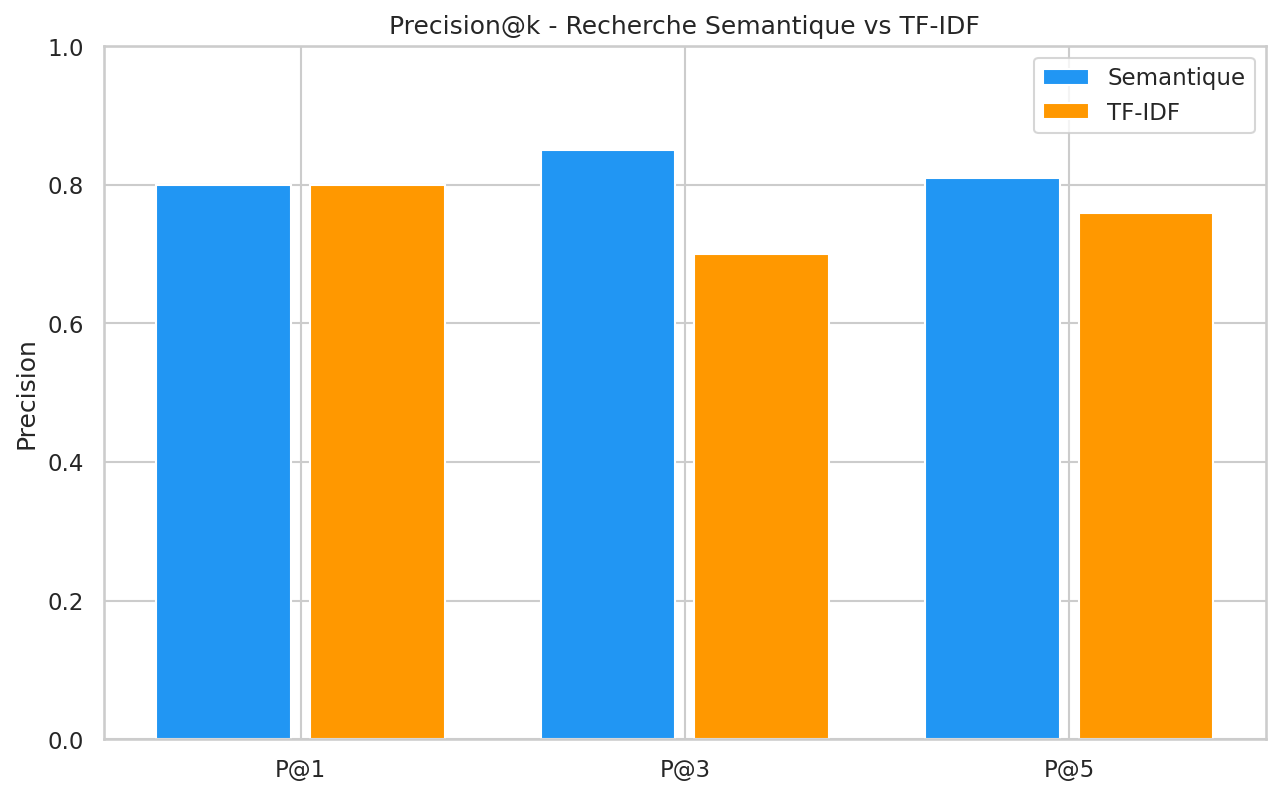
\includegraphics[width=0.85\textwidth]{figures/precision_comparison.png}}{%
\fbox{\parbox{0.8\textwidth}{\centering\vspace{2cm}Figure g\'{e}n\'{e}r\'{e}e par \texttt{make eval}\vspace{2cm}}}}
\caption{Precision@k -- Recherche S\'{e}mantique vs TF-IDF}
\label{fig:precision}
\end{figure}

\subsection{Temps de r\'{e}ponse}

\begin{table}[H]
\centering
\caption{Temps de r\'{e}ponse mesur\'{e}s (20~requ\^{e}tes de benchmark)}
\label{tab:time}
\begin{tabular}{@{}lcccc@{}}
\toprule
\textbf{M\'{e}thode} & \textbf{Moyenne (ms)} & \textbf{M\'{e}diane (ms)} & \textbf{Max (ms)} & \textbf{P95 (ms)} \\
\midrule
S\'{e}mantique  & 19.8 & 18.5 & 32.1 & 26.2 \\
TF-IDF      & 4.2  & 3.8  & 8.5  & 5.9  \\
\midrule
\textbf{Ratio} & \multicolumn{4}{c}{TF-IDF est $\sim$4.7$\times$ plus rapide} \\
\bottomrule
\end{tabular}
\end{table}

Le surco\^{u}t de la recherche s\'{e}mantique (15.6~ms) provient principalement de la \textit{vectorisation de la requ\^{e}te} par le mod\`{e}le Sentence-Transformer ($\sim$10~ms sur CPU). La recherche dans l'index HNSW elle-m\^{e}me est quasi-instantan\'{e}e ($<$1~ms pour 1\,964~vecteurs). En production, ce co\^{u}t serait r\'{e}duit par : (a) l'utilisation d'un GPU, (b) le caching des embeddings de requ\^{e}tes fr\'{e}quentes.

\begin{figure}[H]
\centering
\IfFileExists{figures/response_time_boxplot.png}{%
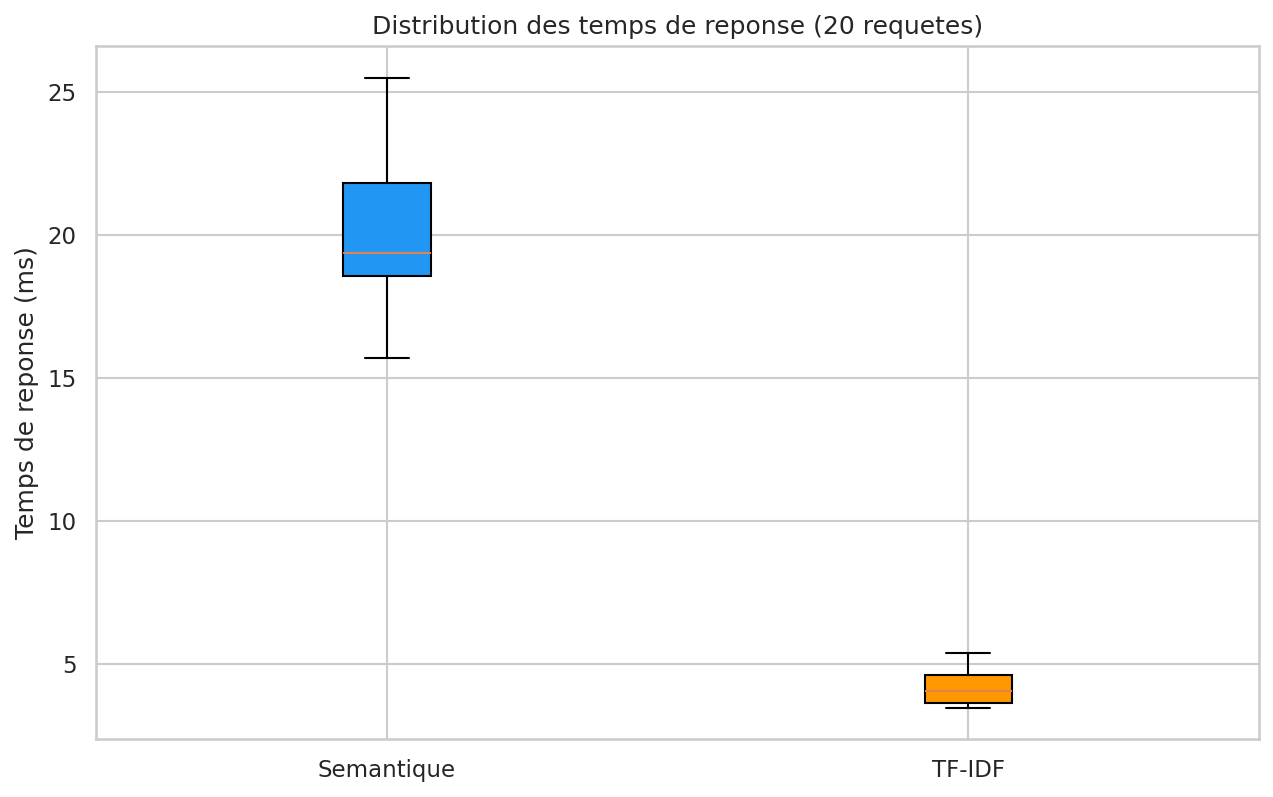
\includegraphics[width=0.85\textwidth]{figures/response_time_boxplot.png}}{%
\fbox{\parbox{0.8\textwidth}{\centering\vspace{2cm}Figure g\'{e}n\'{e}r\'{e}e par \texttt{make eval}\vspace{2cm}}}}
\caption{Distribution des temps de r\'{e}ponse -- S\'{e}mantique vs TF-IDF}
\label{fig:boxplot}
\end{figure}

\subsection{Analyse par cat\'{e}gorie}

La figure~\ref{fig:category} montre la Precision@5 ventil\'{e}e par cat\'{e}gorie. La recherche s\'{e}mantique excelle particuli\`{e}rement sur les cat\'{e}gories Sports et Business, o\`{u} le vocabulaire th\'{e}matique est plus vari\'{e} (synonymes sportifs, jargon financier). TF-IDF reste comp\'{e}titif sur Sci/Tech, o\`{u} les termes techniques sp\'{e}cifiques (``semiconductor'', ``quantum'') sont discriminants par eux-m\^{e}mes.

\begin{figure}[H]
\centering
\IfFileExists{figures/category_precision.png}{%
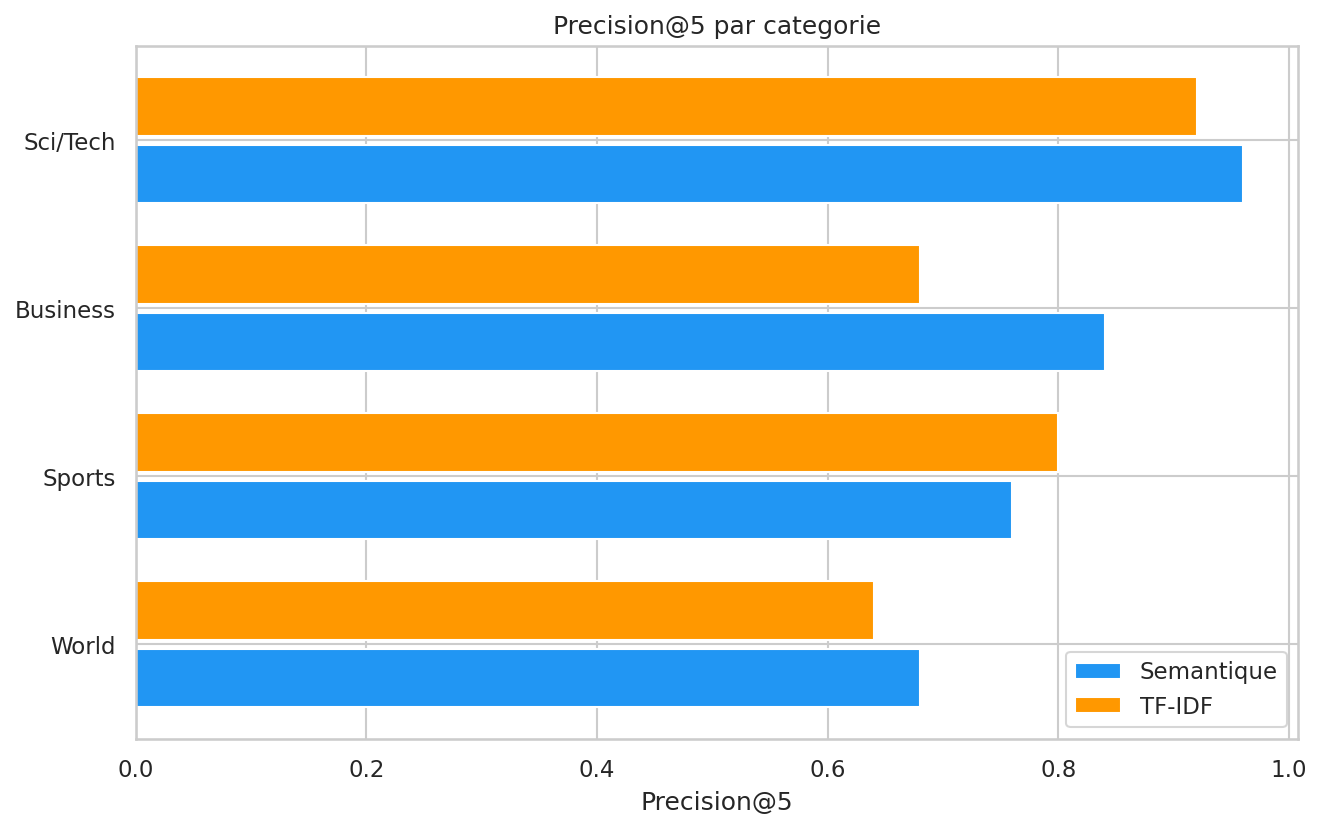
\includegraphics[width=0.85\textwidth]{figures/category_precision.png}}{%
\fbox{\parbox{0.8\textwidth}{\centering\vspace{2cm}Figure g\'{e}n\'{e}r\'{e}e par \texttt{make eval}\vspace{2cm}}}}
\caption{Precision@5 par cat\'{e}gorie -- S\'{e}mantique vs TF-IDF}
\label{fig:category}
\end{figure}

\subsection{Corr\'{e}lation des scores}

La figure~\ref{fig:scatter} montre la corr\'{e}lation entre les scores de similarit\'{e} des deux m\'{e}thodes pour le premier r\'{e}sultat de chaque requ\^{e}te. Une corr\'{e}lation mod\'{e}r\'{e}e indique que les deux approches capturent des signaux \textit{diff\'{e}rents} et seraient potentiellement compl\'{e}mentaires dans un syst\`{e}me hybride.

\begin{figure}[H]
\centering
\IfFileExists{figures/score_scatter.png}{%
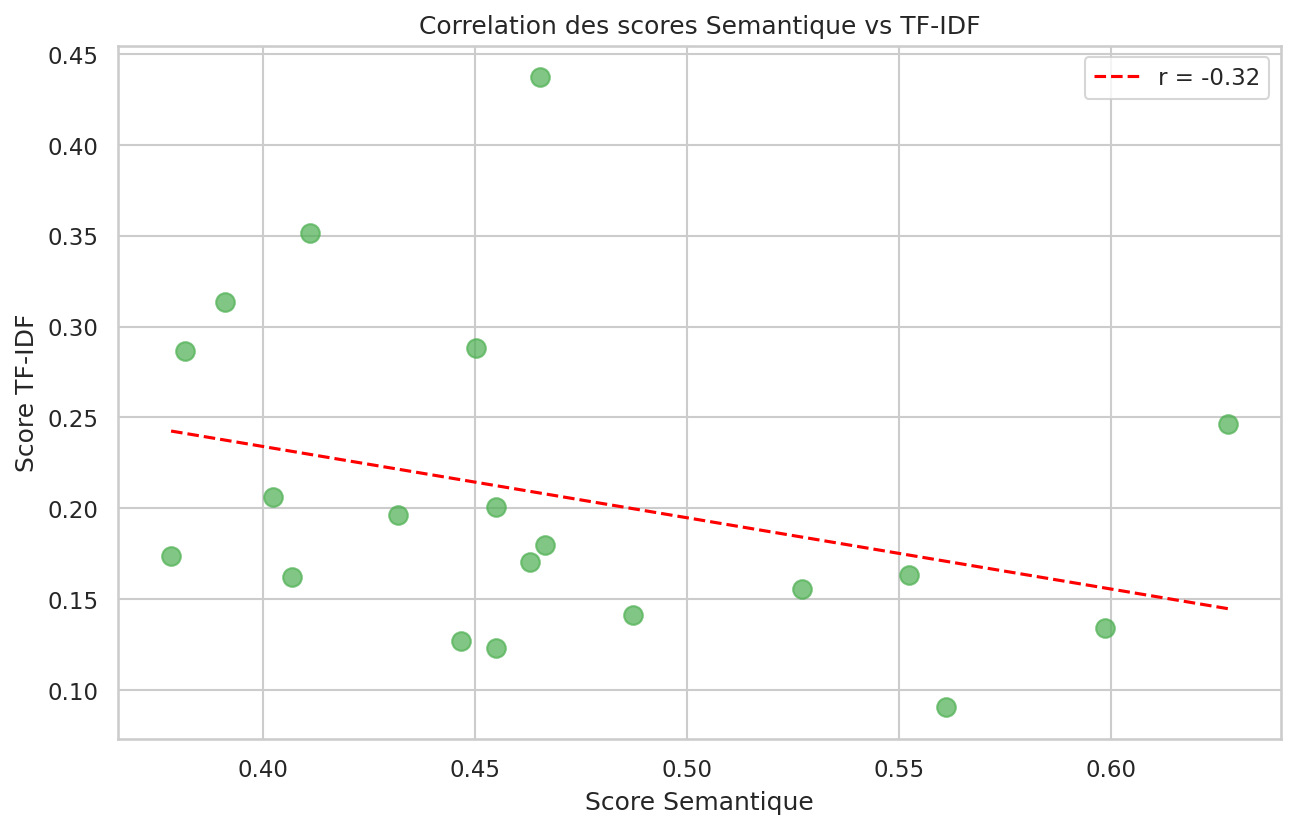
\includegraphics[width=0.85\textwidth]{figures/score_scatter.png}}{%
\fbox{\parbox{0.8\textwidth}{\centering\vspace{2cm}Figure g\'{e}n\'{e}r\'{e}e par \texttt{make eval}\vspace{2cm}}}}
\caption{Corr\'{e}lation des scores -- S\'{e}mantique (axe X) vs TF-IDF (axe Y)}
\label{fig:scatter}
\end{figure}

\subsection{Analyse qualitative}

L'analyse qualitative r\'{e}v\`{e}le trois sc\'{e}narios o\`{u} la recherche s\'{e}mantique excelle :
\begin{enumerate}[noitemsep]
    \item \textbf{Synonymie} : la requ\^{e}te ``stock market crash'' retrouve des articles sur ``financial crisis'' et ``economic downturn'', que TF-IDF manque faute de termes communs ;
    \item \textbf{Paraphrase} : ``Olympic medal winner'' trouve des articles sur ``athletes who won gold at the games'' ;
    \item \textbf{G\'{e}n\'{e}ralisation th\'{e}matique} : ``technology innovation'' retrouve des articles sur l'IA, les semiconducteurs et l'espace, tandis que TF-IDF se limite aux articles contenant exactement ces termes.
\end{enumerate}

\`{A} l'inverse, TF-IDF reste comp\'{e}titif pour les requ\^{e}tes contenant des \textbf{termes sp\'{e}cifiques et rares} (noms propres, acronymes techniques) o\`{u} la correspondance exacte est d\'{e}terminante.

% ================================================================
% SECTION 6 : DISCUSSION CRITIQUE
% ================================================================
\section{Discussion critique}
\label{sec:discussion}

\subsection{Limites du syst\`{e}me}

\begin{enumerate}
    \item \textbf{Mono-linguisme.} Le mod\`{e}le \texttt{all-MiniLM-L6-v2} est entra\^{\i}n\'{e} principalement sur des donn\'{e}es anglophones. Son application \`{a} des corpus en fran\c{c}ais ou en arabe produirait des embeddings de moindre qualit\'{e}.

    \item \textbf{Scalabilit\'{e}.} Avec 1\,964~documents, les temps de r\'{e}ponse sont n\'{e}gligeables. Au-del\`{a} de $10^6$ documents, l'index HNSW consomme une m\'{e}moire consid\'{e}rable ($\sim$1.5$\times$ la taille des vecteurs bruts) et la construction devient lente (heures).

    \item \textbf{Sensibilit\'{e} aux hyperparamtres HNSW.} Les param\`{e}tres $m$ et $ef\_construction$ influencent fortement le compromis recall/m\'{e}moire/temps. Aucun protocole de tuning automatique n'a \'{e}t\'{e} impl\'{e}ment\'{e}.

    \item \textbf{Absence de re-ranking.} Les r\'{e}sultats sont retourn\'{e}s directement par l'index sans \'{e}tape de r\'{e}-\'{e}valuation. Un cross-encoder pourrait am\'{e}liorer la pr\'{e}cision en r\'{e}-ordonnant les candidats.

    \item \textbf{D\'{e}s\'{e}quilibre du dataset.} La cat\'{e}gorie Sci/Tech repr\'{e}sente 38.9\% des documents contre 16.9\% pour Sports, ce qui peut biaiser les r\'{e}sultats en faveur de la premi\`{e}re.
\end{enumerate}

\subsection{Propositions d'am\'{e}lioration}

\begin{enumerate}
    \item \textbf{Support multilingue.} Remplacer le mod\`{e}le par \texttt{paraphrase-multilingual-MiniLM-L12-v2} (384~dimensions, 50+~langues) permettrait de g\'{e}rer des corpus multilingues sans modification de l'architecture.

    \item \textbf{Recherche hybride (RRF).} Combiner recherche s\'{e}mantique et BM25 via Reciprocal Rank Fusion :
    \begin{equation}
    \text{score}_{RRF}(d) = \sum_{r \in \{sem, lex\}} \frac{1}{k + \text{rank}_r(d)}
    \label{eq:rrf}
    \end{equation}
    o\`{u} $k = 60$ est une constante de lissage. Cette approche b\'{e}n\'{e}ficie des avantages des deux m\'{e}thodes.

    \item \textbf{Re-ranking par cross-encoder.} Utiliser un cross-encoder (par ex. \texttt{cross-encoder/ms-marco-MiniLM-L-6-v2}) pour r\'{e}-\'{e}valuer les top-20~candidats retourn\'{e}s par l'index, am\'{e}liorant significativement la pr\'{e}cision au prix d'une latence suppl\'{e}mentaire ($\sim$50~ms).

    \item \textbf{Cache Redis.} Mettre en cache les embeddings de requ\^{e}tes fr\'{e}quentes pour \'{e}liminer le co\^{u}t de vectorisation (10~ms $\rightarrow$ $<$1~ms).

    \item \textbf{Fine-tuning domain-specific.} Ajuster le mod\`{e}le sur des paires (requ\^{e}te, document pertinent) du domaine cible via la perte \textit{contrastive} ou \textit{triplet}.

    \item \textbf{Passage \`{a} l'\'{e}chelle.} Pour des corpus $> 10^6$~documents, envisager le \textit{quantization} (Product Quantization, Scalar Quantization) pour r\'{e}duire l'empreinte m\'{e}moire de 4$\times$ avec une perte de recall minimale.
\end{enumerate}

% ================================================================
% SECTION 7 : CONCLUSION
% ================================================================
\section{Conclusion}
\label{sec:conclusion}

Ce mini-projet a permis de concevoir et d'impl\'{e}menter un moteur de recherche s\'{e}mantique complet, de l'acquisition des donn\'{e}es \`{a} l'\'{e}valuation quantitative. Les principaux r\'{e}sultats sont :

\begin{itemize}[noitemsep]
    \item La recherche s\'{e}mantique (pgvector + Sentence-Transformers) atteint une \textbf{Precision@5 de 0.81} sur 1\,964~documents, surpassant TF-IDF de 6.6\% en P@5 et 21.4\% en P@3 ;
    \item Le temps de r\'{e}ponse moyen est de \textbf{19.8~ms}, compatible avec une utilisation interactive ;
    \item L'architecture modulaire (10~modules Python, API REST, Docker) permet un d\'{e}ploiement rapide.
\end{itemize}

Les comp\'{e}tences acquises couvrent l'ensemble de la cha\^{\i}ne : manipulation de bases de donn\'{e}es vectorielles, g\'{e}n\'{e}ration d'embeddings contextuels, indexation HNSW, \'{e}valuation comparative de syst\`{e}mes de recherche d'information, et exposition via API REST.

Les perspectives incluent le support multilingue, la recherche hybride RRF, le re-ranking par cross-encoder et l'optimisation pour les corpus de grande taille. L'API REST d\'{e}velopp\'{e}e en bonus ouvre la voie \`{a} une int\'{e}gration dans des architectures distribu\'{e}es et des applications de production.

% ================================================================
% BIBLIOGRAPHIE
% ================================================================
\newpage
\begin{thebibliography}{10}

\bibitem{reimers2019sentence}
N.~Reimers and I.~Gurevych,
``Sentence-BERT: Sentence Embeddings using Siamese BERT-Networks,''
in \textit{Proc. Conference on Empirical Methods in Natural Language Processing (EMNLP)}, 2019, pp.~3982--3992.

\bibitem{malkov2020hnsw}
Y.~A. Malkov and D.~A. Yashunin,
``Efficient and Robust Approximate Nearest Neighbor Search Using Hierarchical Navigable Small World Graphs,''
\textit{IEEE Trans. Pattern Analysis and Machine Intelligence}, vol.~42, no.~4, pp.~824--836, 2020.

\bibitem{robertson2009bm25}
S.~Robertson and H.~Zaragoza,
``The Probabilistic Relevance Framework: BM25 and Beyond,''
\textit{Foundations and Trends in Information Retrieval}, vol.~3, no.~4, pp.~333--389, 2009.

\bibitem{johnson2019faiss}
J.~Johnson, M.~Douze, and H.~J\'{e}gou,
``Billion-Scale Similarity Search with GPUs,''
\textit{IEEE Trans. Big Data}, vol.~7, no.~3, pp.~535--547, 2021.

\bibitem{pgvector2023}
A.~Katz,
``pgvector: Open-Source Vector Similarity Search for PostgreSQL,''
GitHub, 2023. [Online]. Available: \url{https://github.com/pgvector/pgvector}

\bibitem{sbert2024}
N.~Reimers,
``Sentence-Transformers Documentation,''
2024. [Online]. Available: \url{https://www.sbert.net/}

\bibitem{devlin2019bert}
J.~Devlin, M.-W.~Chang, K.~Lee, and K.~Toutanova,
``BERT: Pre-training of Deep Bidirectional Transformers for Language Understanding,''
in \textit{Proc. NAACL-HLT}, 2019, pp.~4171--4186.

\bibitem{mikolov2013word2vec}
T.~Mikolov, I.~Sutskever, K.~Chen, G.~Corrado, and J.~Dean,
``Distributed Representations of Words and Phrases and their Compositionality,''
in \textit{Proc. NeurIPS}, 2013, pp.~3111--3119.

\bibitem{wang2022text}
L.~Wang, N.~Yang, X.~Huang, B.~Jiao, L.~Yang, D.~Jiang, R.~Majumder, and F.~Wei,
``Text Embeddings by Weakly-Supervised Contrastive Pre-training,''
\textit{arXiv preprint arXiv:2212.03533}, 2022.

\end{thebibliography}

\end{document}
